%\documentclass[handout]{beamer}
\documentclass{beamer}

\usepackage{amsfonts,amsmath,amsthm,amssymb}
\usepackage{mathtools}
\usepackage{enumitem}
%\usepackage{hyperref}
\usepackage{tikz}
\usepackage{multicol}
\usepackage{bm}
\usepackage[T1]{fontenc}


\usetikzlibrary{calc, matrix, positioning}
\tikzset{ gap/.style = {preaction={draw, line width=2pt, white}} }

\usepackage{helvet}
\usetheme{Madrid}
%\usefonttheme{serif}


\newcommand{\lit}[1]{\textbf{\texttt{#1}}}


\begin{document}

\title{Promise Land}
\subtitle{Proving Correctness with Strongly Typed Javascript-Style Promises}
\author{Andrei Elliott}
\date{May 6, 2022}

\begin{frame}
  \titlepage
\end{frame}

\begin{frame}
  % T.o.C.
  \frametitle\inserttitle
  \tableofcontents
\end{frame}

\section{Introduction}

\begin{frame}
  \centering{\Large \insertsection}
\end{frame}

\begin{frame}
  \frametitle\insertsection
  \begin{itemize}
  \item Javascript Promises
    \begin{itemize}
      \pause\item model for asynchronous code
      \pause\item replaces the ``callback Hell'' of event-driven programming
      \pause\item nicer to use than forks and locks
    \end{itemize}
    \pause\item my contribution
    \begin{itemize}
      \pause\item Haskell library for Promises
      \begin{itemize}
        \pause\item can use Promises from Haskell code
        \pause\item correctness checks JS doesn't have
    \end{itemize}

    \end{itemize}
  \end{itemize}
\end{frame}

\section{Background}

\begin{frame}
  \centering{\Large \insertsection}
\end{frame}

\subsection{Promises}

\begin{frame}
  \frametitle\insertsubsection
  % Promise intro
  \begin{itemize}
  \pause\item adopted in Javascript in ECMAScript 6 standard (2015)
  \pause\item useful, but somewhat error-prone for programmers
  \begin{itemize}
  \pause\item no static checks
  \end{itemize}
  \pause\item use \lit{then} and \lit{next} to attach handlers to a Promise
  \begin{itemize}
    \pause\item handlers run after a Promise has succeeded or failed
    \pause\item result is a new Promise
    \pause\item the computations are said to be \emph{chained} together
  \end{itemize}
\end{itemize}
  %timing diagram
\end{frame}

\begin{frame}
  \frametitle{States of a Promise}
  \begin{center}
  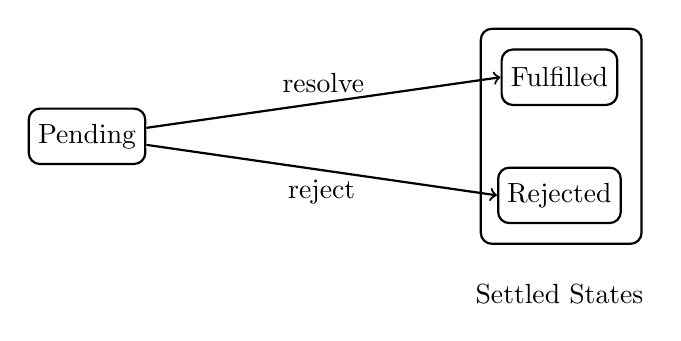
\begin{tikzpicture}
    \path (0,0) node[draw, thick, rounded corners, minimum height=2em, minimum width=4em] (pend) {Pending};
    \pause
    \path (pend)      ++(6,0.75) node[draw, thick, rounded corners, minimum height=2em, minimum width=4em] (ful) {Fulfilled};
    \draw[thick] (pend) edge[gap,->] node[above] {resolve} (ful.west);
    \pause
    \path (pend)  ++(6,-0.75) node[draw, thick, rounded corners, minimum height=2em, minimum width=4em] (rej) {Rejected};
    \draw[thick] (pend) edge[gap,->] node[below] {reject} (rej.west);
    \pause

    \draw[rounded corners, thick] ($(ful.north west)+(-0.25,0.25)$) rectangle ($(rej.south east)+(0.25,-0.25)$);

    \path (rej)  ++(0,-1.25) node {Settled States};
  
\end{tikzpicture}
\end{center}

\end{frame}

\subsection{Haskell}

\begin{frame}
  \frametitle\insertsubsection
  \begin{itemize}
    \pause\item referential transparency
  \pause\item strong type system lets us encode useful information in the types assigned to each value
    \begin{itemize}
    \pause\item automatically checked by the compiler
    \end{itemize}
    \pause\item parameterized types
    \begin{itemize}
      \pause\item abstract over any type
      \pause\item ex: \lit{[a]} is a list whose elements have type \lit a
      \pause\item ex: \lit{Either a b}
      \begin{itemize}
      \item can be a \lit{Left a} or \lit{Right b}
      \pause\item often used as result of a computation that could fail
      \end{itemize}
    \end{itemize}
\end{itemize}

\end{frame}

\begin{frame}
  \frametitle{Monads}
  \begin{itemize}
  \pause\item typeclass grouping types with similar behavior
  \pause\item parameterized by one type
  \pause\item \lit{return}
  \begin{itemize}
  \item \lit{::\ a -> m a}
    \pause  \item puts an arbitrary value into a default context
  \end{itemize}
  \pause\item \lit{(>>=)}
  \begin{itemize}
  \item \lit{::\ m a -> (a -> m b) -> m b}
    \pause\item combines a monadic value with a function that returns a monad
  \end{itemize}
  \pause\item ex: \lit{Either a}
  \begin{itemize}
    \pause\item \lit{return = Right}
    \pause\item \lit{(Right x) >>= f = f x}
    \item \lit{(Left y) >>= f = y}
  \end{itemize}
  \end{itemize}
\end{frame}

\begin{frame}
  \begin{block}{}
    Haskell is referrentially transparent, so how do we represent side effects?
  \end{block}
  \pause
  \begin{itemize}
  \item \lit{IO a}
    \begin{itemize}
    \item action with possible side effects
    \item results in a value of type \lit a
      \pause\item \lit{IO} is a monad
      \end{itemize}
      \pause
    \item \lit{forkIO}
      \begin{itemize}
      \item runs an \lit{IO ()} in a separate thread
      \end{itemize}
      \pause
    \item \lit{MVar a}
      \begin{itemize}
      \item Thread-safe storage box for up to one value of type \lit a
        \pause
      \item \lit{newEmptyMVar ::\ IO (MVar a)}
        \pause
      \item \lit{putMVar ::\ MVar a -> a -> IO ()}
        \pause
      \item \lit{takeMVar ::\ MVar a -> IO a}
      \end{itemize}
  \end{itemize}
\end{frame}

\section{Implementation}

\begin{frame}
  \centering{\Large \insertsection}
\end{frame}


\subsection{Making Promises}

\begin{frame}
  \frametitle\insertsubsection
  \begin{itemize}
    \pause\item Store an \lit{MVar (Either f p)}
    \pause\item \lit{data Promise ::\ * -> * -> * where\\
      \qquad\  Pending ::\ MVar (Either f p) -> Promise f p}
    \pause\item\item JS version accepts an \emph{executor} function
    \begin{itemize}
    \pause\item two callbacks: for success and failure
  \end{itemize}
  \pause\item\item use: \lit{newPromise ($\lambda$ s f -> if error then f("Failed!")\\
    \qquad \qquad else s(value))}
  \end{itemize}

\end{frame}

\begin{frame}
  \frametitle{newPromise}
  
   Type:\\
  \begin{align*}
  \lit{\only<-2>{executor}\only<3>{(successFun -> failFun -> ?)}\only<4->{((p -> IO ()) -> (f -> IO ()) -> IO ())} -> \only<2->{IO} (Promise f
      p)}
  \end{align*}\\
  \onslide<5> {Code:\\
  \lit{newPromise k = do\\
 \qquad  state <- newEmptyMVar\\
 \qquad forkIO \$ k (putMVar state . Right) \\
 \qquad \qquad \qquad \ \ \  (putMVar state . Left)\\
   \qquad return (Pending state)}}

\end{frame}

\subsection{Then What?}

\begin{frame}
  \frametitle\insertsubsection
  \begin{itemize}
    \pause\item \lit{then} registers a callback to a succeeding Promise
    \pause\item accepts a Promise and a function that creates a new Promise from a success value
    \pause\item \lit{pThen ::\ Promise f p\\
\qquad        -> (p -> IO (Promise f p'))\\
\qquad        -> IO (Promise f p')
}
  \end{itemize}
\end{frame}

\subsection{Parallel Promises}
%pRace2
\begin{frame}
  \frametitle\insertsubsection
  \begin{itemize}
    \pause\item various ways to combine Promises to run in parallel
    \pause\item ex: \lit{race}
    \begin{itemize}
    \item runs a list of input Promises
      \pause\item stops when the first one settles
    \item settles with that value
      \pause\item \lit{pRace :: [Promise f p] -> IO (Promise f p)}
      \end{itemize}
  \end{itemize}
\end{frame}

\subsection{Monad Instance}
\begin{frame}
  \frametitle\insertsubsection
  \begin{itemize}
    \pause \item \lit{instance Monad (Promise f)}
    \pause\item \lit{return} is the function \lit{resolve}
    \begin{itemize}
    \item creates a Promise that succeeds immediately
    \end{itemize}
    \pause\item \lit{(>>=)} for \lit{Promise f} has type
    \begin{itemize}
    \item \lit{Promise f a -> (a -> Promise f b) -> Promise f b}
    \pause\item looks a lot like \lit{pThen}
    \pause\item but \lit{pThen} results in an \lit{IO (Promise f b)}
    \pause\item extra Promise constructor storing the callback
    \begin{itemize}
    \item uses \lit{pThen} when we run the Promise
    \end{itemize}
    \end{itemize}
  \end{itemize}
\end{frame}

\section{Results}

\begin{frame}
  \centering{\Large \insertsection}
\end{frame}


\begin{frame}
  \begin{block}{}
    Would the sytem detect real bugs?
  \end{block}
  \begin{itemize}
    \pause\item Madsen et al. (2017) case study
    \begin{itemize}
      \pause\item 21 Stack Overflow questions about JS Promises
      \pause\item 6: unintentional \lit{undefined} \pause {\huge \checkmark}
      \pause\item 3: dead Promise \only<11>{{\huge \checkmark}}
      \begin{itemize}
        \pause\item executor never calls either callback
        \pause\item Promise is \emph{Pending} forever
        \pause\item catch these by updating the type of \lit{newPromise}
      \end{itemize}
    \end{itemize}
    \pause\item\item\lit{((p -> IO Token) -> (f -> IO Token) -> IO Token)\\
        \qquad  -> IO (Promise f p)}
  \end{itemize}
  % what can we prove with the types?
  % 'Void trick' to detect dead promises
\end{frame}

\begin{frame}
  \center \huge Thank You
\end{frame}

\end{document}
